\documentclass{article}
% Language setting
% Replace `english' with e.g. `spanish' to change the document language
\usepackage[english]{babel}
% Set page size and margins
% Replace `letterpaper' with `a4paper' for UK/EU standard size
\usepackage[letterpaper,top=2cm,bottom=2cm,left=3cm,right=3cm,marginparwidth=1.75cm]{geometry}
% Useful packages
\usepackage{multicol}
\usepackage{amsmath}
\usepackage{amssymb}
\usepackage{graphicx}
\usepackage[framemethod=tikz]{mdframed}
\usepackage{array}
\usepackage{blindtext}
%\usepackage[paperwidth=10cm]{geometry}
\usepackage{tkz-euclide}
%\usepackage{tikz}
\usetikzlibrary{
  circuits.logic,
  circuits.logic.US,
  positioning
}

\usepackage[colorlinks=true, allcolors=blue]{hyperref}
\newcommand{\myvec}[1]{\ensuremath{\begin{pmatrix}#1\end{pmatrix}}}
\providecommand{\norm}[1]{\left\lVert#1\right\rVert}
\let\vec\mathbf
\title{Optimization Assignment-1}
\author{Ballepu dheeraj kumar}
\begin{document}
\maketitle
\newtheorem{theorem}{Theorem}[section]
\begin{multicols}{2}

\paragraph{\begin{flushleft}\textbf{Problem: }
\textbf{Minimise and Maximise}
\begin{align*}
Z = 5x+10y
\end{align*}
subjected to
\begin{align*}
x+2y \preceq 120, x+y \succeq 60, x-2y \succeq 0, x \succeq 0 , y \succeq 0
\end{align*}
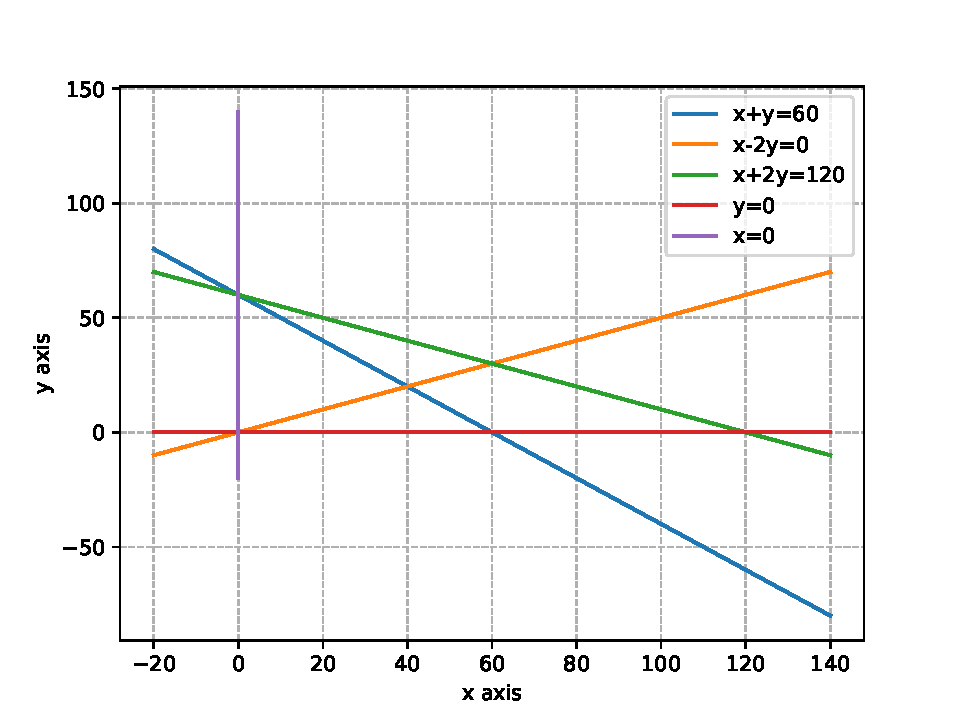
\includegraphics[scale=0.5]{/sdcard/Download/Opti/figure2/opt1.pdf} 
\end{flushleft}}
\section*{Solution}
\begin{flushleft}
Problem can be formulated as,\\
\end{flushleft}
\begin{align}
\min_{\vec{x}} Z=(5x+10y)\\
\max_{\vec{x}} Z=(5x+10y)
\end{align}
\begin{align*}
x+2y \preceq 120
\end{align*}
\begin{align*}
x+y \succeq 60
\end{align*}
\begin{align*}
x-2y \succeq 60
\end{align*}
\begin{align*}
x \succeq 0 , y \succeq 0
\end{align*}
all the above expressions can be expressed in vector form as
\begin{align*}
\min_{\vec{x}}\vec{Z}=\myvec{5 \hspace{0.2cm}10}\vec{x}\\
\max_{\vec{x}}\vec{Z}=\myvec{5 \hspace{0.2cm}10}\vec{x}\\
\myvec{1 \hspace{0.2cm}1\\
       1 \hspace{0.2cm}-2\\
       1 \hspace{0.2cm}0\\
       0 \hspace{0.2cm}1}\vec{x}\succeq \myvec{60 \\0\\0\\0}\\   
 \myvec{1 \hspace{0.2cm}2}\vec{x}\preceq \myvec{120}  
\end{align*}
%\begin{align}
%\max_{\vec{x}}\vec{Z}=\myvec{5 \hspace{0.2cm}10}\vec{x}\\
%\myvec{1 \hspace{0.2cm}2\vec{x}\preceq \myvec{120}
%\end{align}
Solving above equations using cvxpy, we get\\
\vspace{0.1cm}\\
\begin{align}
\min_{\vec{x}} Z=300
\end{align}
\begin{align}
\vec{x}=\myvec{60\\0}
\end{align}
\vspace{0.1cm}\\
\begin{align}
\max_{\vec{x}} Z=600
\end{align}
\begin{align}
\vec{x}=\myvec{60\\30}
\end{align}
\end{multicols}{2}
\end{document}
